\section{Some commonly encountered problems}
\label{SectCommProblem}

\subsection{1. The version of Maven and Maven plugins do matter}
\textbf{We highly recommend using Maven 3.1.1.}

In addition, according to tests, not all versions of Maven and Maven release plugins are compatible.
Some test results:
\begin{verbatim}
Maven 3.2.3 + maven-release-plugin 2.5 = SUCCESS
Maven 3.1.1 + maven-release-plugin 2.2.1 =SUCCESS
Maven 3.2.3 + maven-release-plugin 2.2.1 = FAIL
\end{verbatim}


If Maven is not compatible with the release plugin, you may see a message like this:
\begin{qa}
\item[]
(default-cli)  API incompatibility while executing 
\item[]
org.apache.maven.plugins:maven-release-plugin:2.2.1:prepare: 
\item[] java.lang.NoSuchMethodError.
\end{qa}

Additionally, David Klapper proposed to use Maven 2.5
as well as to  force some additional plugins to 1.9.1.
In his opinion, the second part is probably not strictly necessary for us i.e., 
as long as your PoM is in the repository root but just to be sure.

Your PoM file may contain the following:
\begin{verbatim}
<plugin>
    <groupId>org.apache.maven.plugins</groupId>
    <artifactId>maven-release-plugin</artifactId>
    <version>2.5</version>
    <executions>
        <execution>
            <id>default</id>
            <goals>
                <goal>perform</goal>
            </goals>
            <configuration>
                <pomFileName>hw0-ANDREW_ID/pom.xml</pomFileName>
            </configuration>
        </execution>
    </executions>
    <dependencies>
        <dependency>
            <groupId>org.apache.maven.scm</groupId>
            <artifactId>maven-scm-api</artifactId>
            <version>1.9.1</version>
        </dependency>
        <dependency>
            <groupId>org.apache.maven.scm</groupId>
            <artifactId>maven-scm-provider-gitexe</artifactId>
            <version>1.9.1</version>
        </dependency>
    </dependencies>
</plugin>
\end{verbatim}

\subsection{2. Success on course-snapshots but not course-releases}

\begin{qa}
\item[Q] I succeeded to push to course-snapshots, but not to course-releases. 
More specifically, it showed "release success" in the console and showed up on the \url{http://mu.lti.cs.cmu.edu:8081/nexus/content/repositories/course-snapshots/edu/cmu/lti/11791/f14/hw0/}, but I failed to see my artifact in the remote repositories of Course Releases. (\url{http://mu.lti.cs.cmu.edu:8081/nexus/content/repositories/course-releases/edu/cmu/lti/11791/f14/hw0/})  What probably caused this?
\end{qa}

If you cannot figure out the right combination of Maven plugins, you can bump into this issue.
One hacky solution is as follows:
\begin{enumerate}
\item First follow the instructions from the hw0 guide.
\item Remove -SNAPSHOT from the version in pom.xml, commit and push to git, but do not run maven release.
\item Add -SNAPSHOT back to the version. Then run maven release:prepare release:perform.
You may see a "tag already existed" error. Just delete the previous tag from git first.
For tag-deletion instructions see e.g. \url{http://nathanhoad.net/how-to-delete-a-remote-git-tag}.
\end{enumerate}

\subsection{3. Maven executable not found}
Several people failed to release, because Maven wasn't configured properly.
In this case, people see an error message like this:
\begin{qa}
\item[]
[ERROR] Failed to execute goal org.apache.maven.plugins:maven-release-plugin:2.2.1:prepare (default-cli) on project hw0-ANDREWID: Failed to invoke Maven build. Error configuring command-line. Reason: Maven executable not found at: /Users/ANDREWID/Documents/workspace/hw0-ANDREWID/EMBEDDED/bin/mvn $->$ [Help 1]
\end{qa}

First, go to Maven/Preferences/Windows/Installations and check if you replaced the embedded Maven with
an external Maven installation (Please, refer to Figure \ref{submit-02-add-maven}).

Second, when you create a maven build to execute goals ``release:prepare release:perform'',
there is an option to specify a Maven runtime. In our version of Eclipse, 
it was a dropdown menu/list at the bottom of the window,
which appears when you create a new run configuration (of the type Maven build).
So, if you have such an option, make sure you specify
an external Maven rather than an embedded one.

There were cases, when these recommendations did not help. As a last resort, one can invoke
Maven directly. This can be done either from the command line (which is straightforward),
or even from the Eclipse (as suggested by LIU Xi).
To do this, go to Run/External tools/External tools configurations and create a new external run.
A window similar to that in Figure \ref{MavenExtTool} will appear.



\begin{figure}
\centering
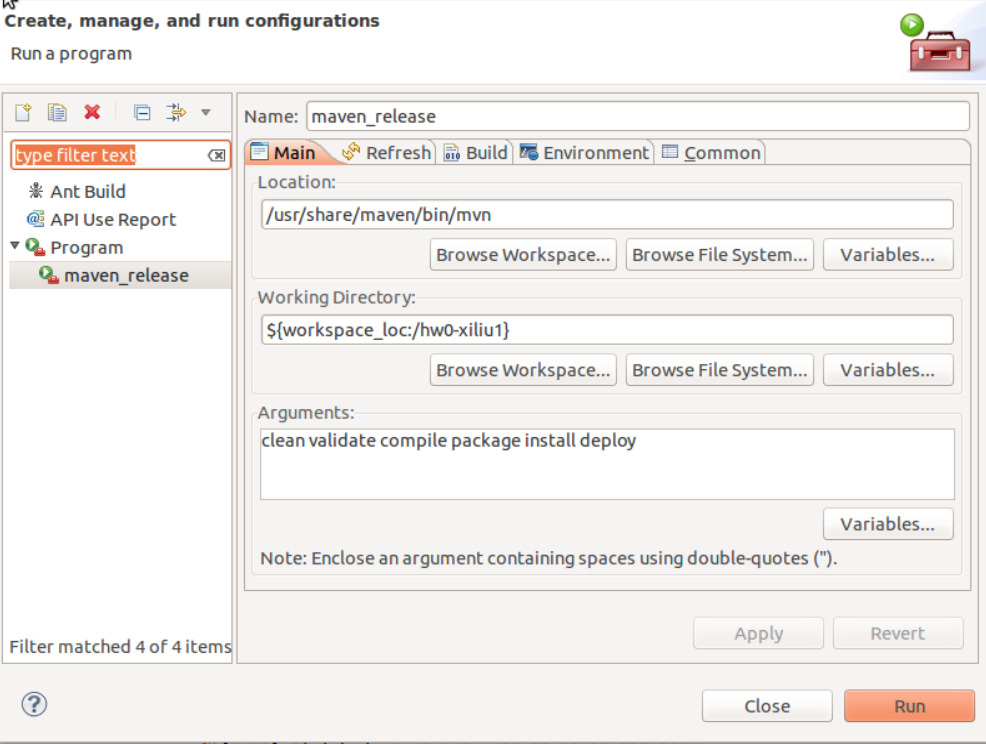
\includegraphics[scale=0.4]{maven_release_as_an_external_tool}
\caption{Invoking Maven as an external tool\label{MavenExtTool}}
\end{figure}

\subsection{4. Cannot tag, because the tag already exits.}
If you repeat an operation multiple times (due to errors),
you may see a message:
\begin{verbatim}
Error: unable to tag scm.  fatal: tag already exits.
\end{verbatim}
\href{http://git-scm.com/docs/git-tag}{Tagging is a labeling mechanism of Git},
which is used by Maven to label specific releases.
The name of the tag is built based on the artifact version
that is specified in the Pom file.
Due to previous unsuccessful operations, the tag has already been created.
Thus, it cannot be recreated again (with the same name).

Two solutions are possible. A good solution is to delete the previously
created tag,
see e.g. \url{http://nathanhoad.net/how-to-delete-a-remote-git-tag}.
Unfortunately, the Maven release plugin cannot do it (though should) on its own.
A hacky and dirty solution is to change the version of the artifact 
in the Pom file so that it does not collide with any of the 
previously created version. 
Bad approach for people working at Google, but, probably, good
enough for you to finish the homework if you are running out of time.

\subsection{5. Cannot tag scm/push to Git, because of the wrong authentication protocol}

You may see an error:
\begin{verbatim}
fatal: cannot push gitxxxxxxxxxxxxxx, try use https://xxxxxxxxxx
\end{verbatim}

As explained previously, one should not use \emph{HTTPS} authentication 
for Maven. Please, check the scm-address in your Pom file.
You should use the \emph{SSH} authentication and the correct scm format 
should be:
\begin{verbatim}
scm:git:git@github.com:GITHUB_ID/hw0-ANDREW_ID.git
\end{verbatim}

\subsection{6. Cannot tag scm, because access is denied}

If you see an error:
\begin{verbatim}
fatal: cannot push gitxxxxxxxxxxxxxx, access denied (publickey)
\end{verbatim}
It is may caused by inappropriate SSH-key setting. Check or reset your SSH-key.

\subsection{7. 
 error:  You don't have a SNAPSHOT project in the reactor projects list.}
If you see the following error:
\begin{verbatim}
 error:  You don't have a SNAPSHOT project in the reactor projects list.
\end{verbatim}
Check your pom.xml, $<$version$>$ tag. Make sure you have -SNAPSHOT suffix link like this: 
\begin{verbatim}
<version>0.0.1-SNAPSHOT</version>
\end{verbatim}

\subsection{8. Cannot push upstream}

In some version of Eclipse (and OS), the option "PUSH TO UPSTREAM" is not available.
One may be able to use \textbf{Remote$->$Push} instead.

\subsection{9. Error parsing Pom file}
The XML can be malformed, even though visually it looks fine.
One common error was encountered on Mac.
Turns out, certain non-printable characters on Mac just never appear on screen:
neither in Eclipse editor nor in Vi.
These pesky characters can be detected using at least three approaches:
\begin{itemize}
\item Check how the file looks at GitHub ideally using your friend's computer (ideally
it should have different locale settings);
\item Clone your repository on one of the Linux machines (you may have access to ScS servers)
and open the file in Vi.
\item Use the command \texttt{hexdump -C pom.xml}.
\end{itemize}

